\newcommand{\rowmetric}[6]{
#1 & % Name
\textcolor{verdun}{#2} & % TCP
\textcolor{cyprus}{#3} & % TCS
\textcolor{derby}{#4} & % TSR
\textcolor{bossanova}{#5} & % TSA
#6 % Description
\\}

\begin{figure}
  \center
  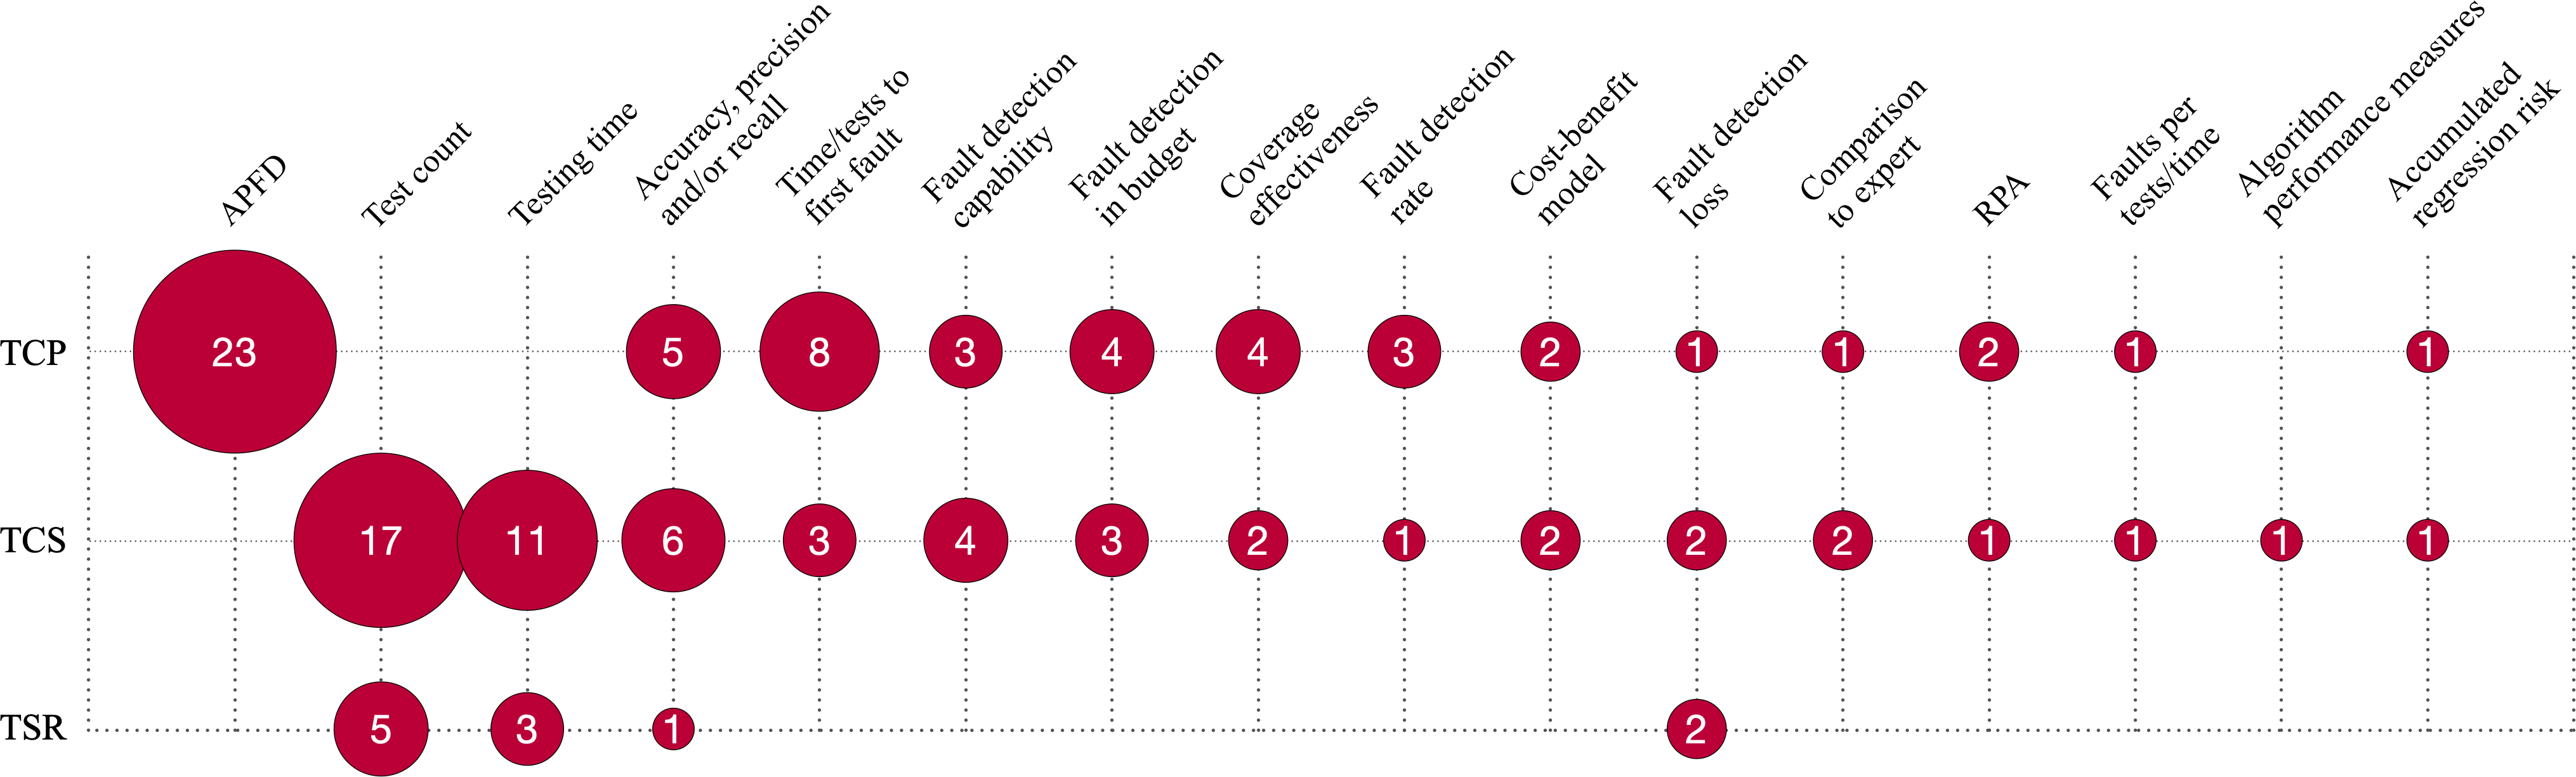
\includegraphics[width=\linewidth]{figures/effectiveness_metrics.pdf}
  \caption{Distribution of effectiveness metrics.}
  \label{fig:effectiveness_metrics}
\end{figure}

\begin{figure}
  \center
  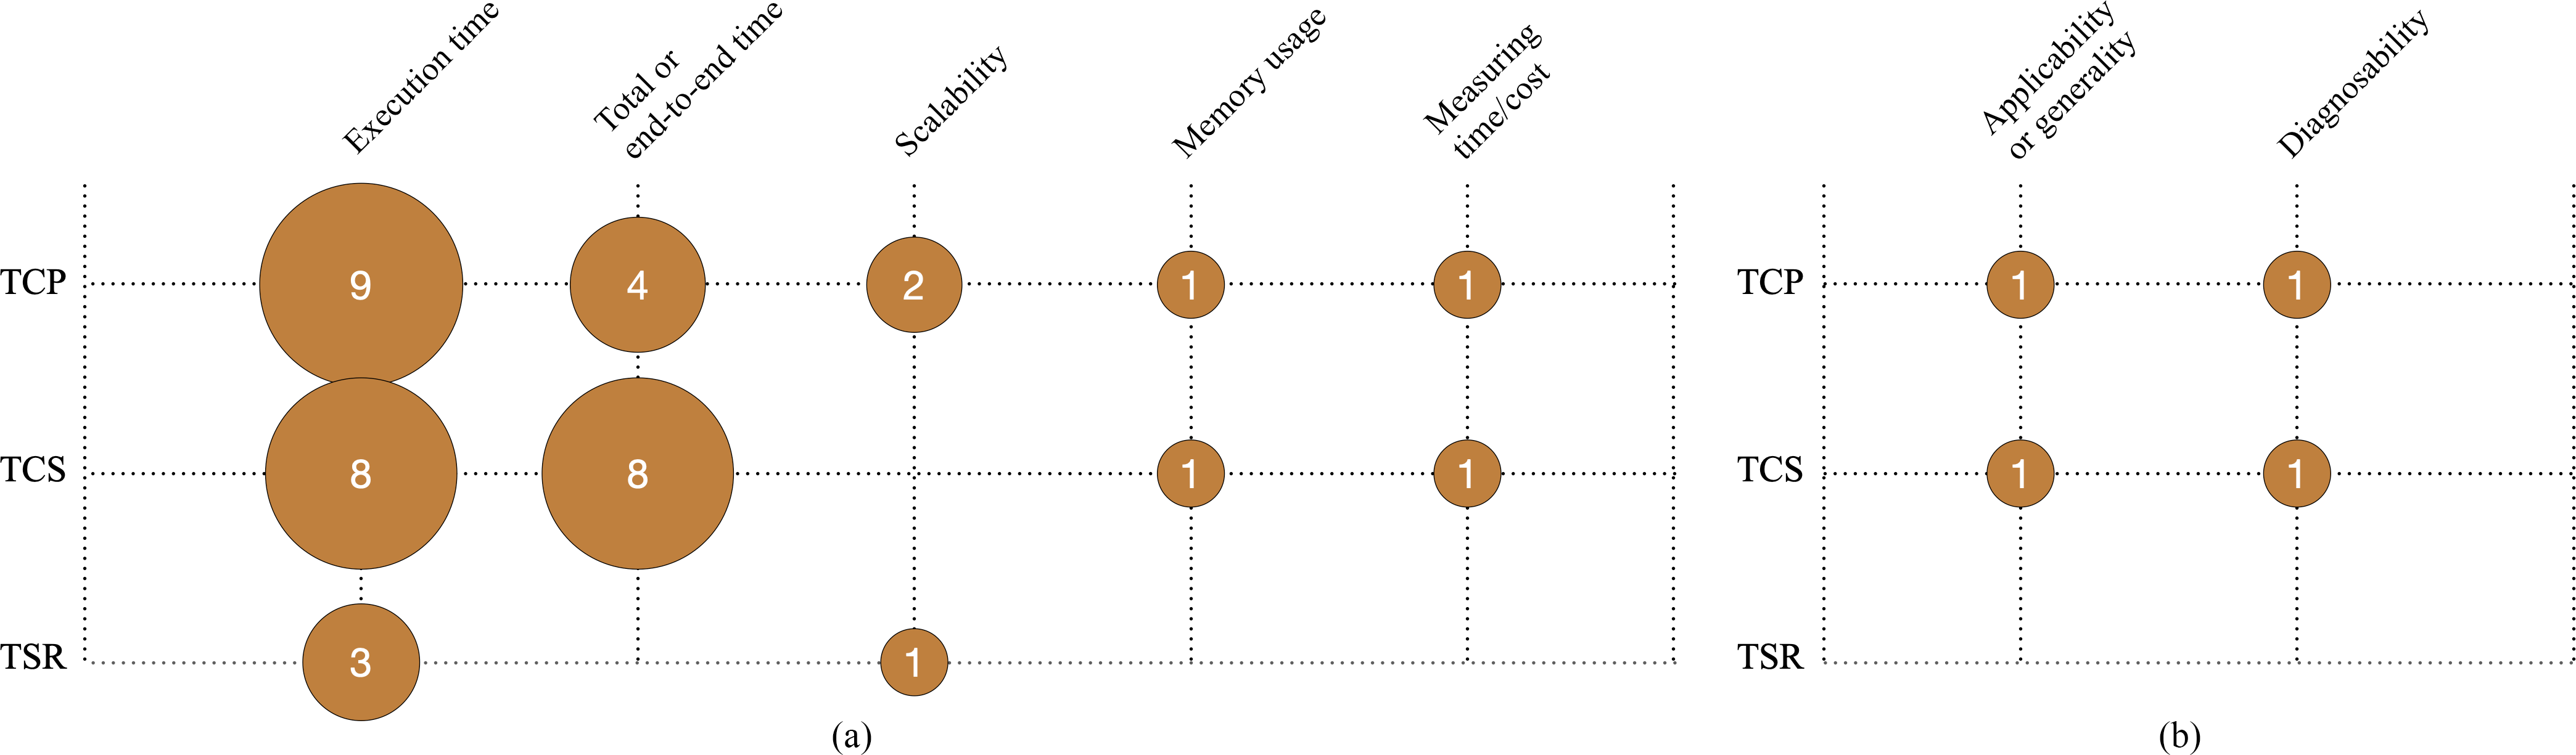
\includegraphics[width=\linewidth]{figures/efficiency_other_metrics.pdf}
  \caption{Distribution of (a) efficiency and (b) other metrics.}
  \label{fig:efficiency_metrics}
\end{figure}

\begin{table}[]
\scriptsize
\centering
\setlength{\tabcolsep}{1,2mm}
\begin{tabular}{p{23mm}p{18mm}p{18mm}p{8mm}p{8mm}p{60mm}}
\toprule
\textbf{Effectiveness} & 
\textcolor{verdun}{\textbf{\tcp}} & 
\textcolor{cyprus}{\textbf{\tcs}} & 
\textcolor{derby}{\textbf{\tsr}} & 
\textcolor{bossanova}{\textbf{\tsa}} & 
\textbf{Description} \\ 
\midrule
\showrowcolors
\rowmetric{Selection/reduction count/percentage}{}{\citetalias{hirzel_graph-walk-based_2016}, \citetalias{vost_trace-based_2016}, \citetalias{blondeau_test_2017}, \citetalias{bach_coverage-based_2017}, \citetalias{vasic_file-level_2017}, \citetalias{celik_regression_2017}, \citetalias{zhang_hybrid_2018}, \citetalias{yilmaz_case_2018}, \citetalias{celik_regression_2018}, \citetalias{azizi_retest_2018}, \citetalias{fu_resurgence_2019}, \citetalias{eda_efficient_2019}, \citetalias{machalica_predictive_2018}, \citetalias{shi_understanding_2019}, \citetalias{chen_context-aware_2021}, \citetalias{zhang_comparing_2022}, \citetalias{cingil_black-box_2022}}{\citetalias{gotlieb_using_2017}, \citetalias{chi_multi-level_2017}, \citetalias{eda_efficient_2019}, \citetalias{goyal_test_2019}, \citetalias{noemmer_evaluation_2020}}{}{Absolute or relative size of the resulting test suite compared to the original.}
\rowmetric{Average Percentage of Faults Detected (APFD)}{\citetalias{srikanth_requirements_2016}, \citetalias{lu_how_2016}, \citetalias{srikanth_test_2016}, \citetalias{busjaeger_learning_2016}, \citetalias{marijan_effect_2016}, \citetalias{spieker_reinforcement_2017}, \citetalias{ouriques_test_2018}, \citetalias{haghighatkhah_test_2018}, \citetalias{miranda_fast_2018}, \citetalias{chen_optimizing_2018}, \citetalias{yu_terminator_2019}, \citetalias{wu_time_2019}, \citetalias{lima_multi-armed_2022}, \citetalias{peng_empirically_2020}, \citetalias{bagherzadeh_reinforcement_2022}, \citetalias{pan_dynamic_2020}, \citetalias{zhou_parallel_2022}, \citetalias{li_aga_2021}, \citetalias{abdelkarim_tcp-net_2022}, \citetalias{yaraghi_scalable_2022}, \citetalias{omri_learning_2022}, \citetalias{greca_comparing_2022}}{}{}{}{A measure of how quickly a test suite detects faults, on average. Includes many variations, such as APFDc and NAPFD.}
\rowmetric{Testing time}{}{\citetalias{tahvili_dynamic_2016}, \citetalias{ramler_tool_2017}, \citetalias{celik_regression_2017}, \citetalias{garousi_multi-objective_2018}, \citetalias{yilmaz_case_2018}, \citetalias{celik_regression_2018}, \citetalias{zhong_testsage:_2019}, \citetalias{shi_understanding_2019}, \citetalias{mehta_data-driven_2021}, \citetalias{zhang_comparing_2022}, \citetalias{cingil_black-box_2022}}{\citetalias{goyal_test_2019}, \citetalias{philip_fastlane:_2019}, \citetalias{noemmer_evaluation_2020}}{}{Time required to execute the prioritized/selected/reduced test suite as opposed to the original suite.}
\rowmetric{Accuracy, precision and recall}{\citetalias{busjaeger_learning_2016}, \citetalias{kwon_cost-effective_2017}, \citetalias{pan_dynamic_2020}, \citetalias{abdelkarim_tcp-net_2022}, \citetalias{omri_learning_2022}}{\citetalias{blondeau_test_2017}, \citetalias{magalhaes_automatic_2016}, \citetalias{kwon_cost-effective_2017}, \citetalias{guo_decomposing_2019}, \citetalias{machalica_predictive_2018}, \citetalias{xu_requirement-based_2021}}{\citetalias{philip_fastlane:_2019}}{}{Measures of correctness and completeness of the resulting test suite (e.g., count of false positives and false negatives).}
\rowmetric{Fault Detection Capability}{\citetalias{schwartz_cost-effective_2016}, \citetalias{wang_enhancing_2016}, \citetalias{marijan_effect_2016}}{\citetalias{kwon_cost-effective_2017}, \citetalias{zarges_artificial_2021}, \citetalias{chen_context-aware_2021}, \citetalias{cingil_black-box_2022}}{}{}{Number or proportion of faults detected by the resulting suite compared to the original.}
\rowmetric{Fault Detection Rate (FDR)}{\citetalias{aman_application_2016}, \citetalias{strandberg_experience_2016}, \citetalias{yu_terminator_2019}}{\citetalias{azizi_retest_2018}}{}{}{Time to detect faults compared to the optimal RT suite.}
\rowmetric{Coverage Effectiveness (CE)}{\citetalias{noor_similarity-based_2016}, \citetalias{yu_terminator_2019}, \citetalias{magalhaes_hsp_2020}, \citetalias{lubke_selecting_2020}}{\citetalias{magalhaes_hsp_2020}, \citetalias{lubke_selecting_2020}}{}{\citetalias{yoshida_fsx_2016}}{Measure of the tradeoff between cost of the test suite and structural coverage of the SUT.}
\rowmetric{Time/tests To First Failure}{\citetalias{noor_similarity-based_2016}, \citetalias{chen_optimizing_2018}, \citetalias{zhu_test_2018}, \citetalias{lima_multi-armed_2022}, \citetalias{zhou_beating_2020}, \citetalias{pan_dynamic_2020}, \citetalias{zhou_parallel_2022}, \citetalias{greca_comparing_2022}}{\citetalias{blondeau_test_2017}, \citetalias{zarges_artificial_2021}, \citetalias{greca_comparing_2022}}{}{}{Number of tests or amount of time needed to reach the first failure.}
\rowmetric{Fault detection within a budget}{\citetalias{wang_enhancing_2016}, \citetalias{bach_coverage-based_2017}, \citetalias{lima_multi-armed_2022}, \citetalias{greca_comparing_2022}}{\citetalias{pradhan_search-based_2016}, \citetalias{bach_coverage-based_2017}, \citetalias{greca_comparing_2022}}{}{}{Faults still detected when restricting the testing time budget.}
\rowmetric{Cost-benefit model}{\citetalias{schwartz_cost-effective_2016}, \citetalias{tahvili_cost-benefit_2016}}{\citetalias{garousi_multi-objective_2018}, \citetalias{mehta_data-driven_2021}}{}{}{Mathematical models considering costs and benefits of applying a technique throughout development.}
\rowmetric{Fault Detection Loss}{\citetalias{najafi_improving_2019}}{\citetalias{najafi_improving_2019}, \citetalias{chen_multi-objective_2021}}{\citetalias{shi_evaluating_2018}, \citetalias{cruciani_scalable_2019}}{}{Number or proportion of faults undetected by the selected/reduced test suite compared to the original.}
\rowmetric{Comparison to expert}{\citetalias{buchgeher_improving_2016}}{\citetalias{buchgeher_improving_2016}, \citetalias{magalhaes_automatic_2016}}{}{}{Compares the output of the tool with a list of tests selected by the project architect.}
\rowmetric{Faults per tests or time}{\citetalias{kwon_cost-effective_2017}}{\citetalias{kwon_cost-effective_2017}}{}{}{Number of faults deteted per number of tests or testing time.}
\rowmetric{Number of tests added}{}{}{}{\citetalias{yoshida_fsx_2016}}{Number of tests added to the test suite.}
\rowmetric{Algorithm performance measures}{}{\citetalias{pradhan_search-based_2016}}{}{}{Fitness value or hypervolume metrics applied to search-based algorithms}
\rowmetric{Accumulated regression risk}{\citetalias{lubke_selecting_2020}}{\citetalias{lubke_selecting_2020}}{}{}{How much of the "regression risk" is covered by the tests.}
\rowmetric{Rank Percentile Average (RPA)}{\citetalias{bertolino_learning--rank_2020}, \citetalias{bagherzadeh_reinforcement_2022}}{\citetalias{bertolino_learning--rank_2020}}{}{}{Comparison between the predicted ranking and the actual ranking (from the dataset).}
\hiderowcolors
\bottomrule

%\end{tabular}
%\caption{Effectiveness Metrics}	
%\label{table:effectiveness_metrics}
%\end{table}
%
%\begin{table}[]
%\scriptsize
%\centering
%\begin{tabular}{p{25mm}p{15mm}p{15mm}p{8mm}p{8mm}p{60mm}}
%\toprule
\textbf{Efficiency} & 
\textcolor{verdun}{\textbf{\tcp}} & 
\textcolor{cyprus}{\textbf{\tcs}} & 
\textcolor{derby}{\textbf{\tsr}} & 
\textcolor{bossanova}{\textbf{\tsa}} & 
\textbf{Description} \\ \midrule
\showrowcolors
\rowmetric{Execution time}{\citetalias{wang_enhancing_2016}, \citetalias{haghighatkhah_test_2018}, \citetalias{miranda_fast_2018}, \citetalias{najafi_improving_2019}, \citetalias{wu_time_2019}, \citetalias{lima_multi-armed_2022}, \citetalias{zhou_parallel_2022}, \citetalias{li_aga_2021}, \citetalias{greca_comparing_2022}}{\citetalias{hirzel_graph-walk-based_2016}, \citetalias{vasic_file-level_2017}, \citetalias{celik_regression_2017}, \citetalias{zhong_testsage:_2019}, \citetalias{najafi_improving_2019}, \citetalias{xu_requirement-based_2021}, \citetalias{zhang_comparing_2022}, \citetalias{greca_comparing_2022}}{\citetalias{gotlieb_using_2017}, \citetalias{chi_multi-level_2017}, \citetalias{cruciani_scalable_2019}}{\citetalias{yoshida_fsx_2016}}{Time required to run the tool (e.g., selection time, prioritization time, etc).}
\rowmetric{Total/End-to-end time}{\citetalias{wang_enhancing_2016}, \citetalias{miranda_fast_2018}, \citetalias{bertolino_learning--rank_2020}, \citetalias{greca_comparing_2022}}{\citetalias{oqvist_extraction-based_2016}, \citetalias{vasic_file-level_2017}, \citetalias{zhang_hybrid_2018}, \citetalias{celik_regression_2018}, \citetalias{fu_resurgence_2019}, \citetalias{bertolino_learning--rank_2020}, \citetalias{zhang_comparing_2022}, \citetalias{greca_comparing_2022}}{}{}{End-to-end time, combining measuring time, execution time and testing time. Due to this, it is a measure of both efficiency and effectiveness.}
\rowmetric{Memory usage}{\citetalias{wang_enhancing_2016}}{\citetalias{hirzel_graph-walk-based_2016}}{}{}{Measures the amount of memory used by the tool.}
\rowmetric{Scalability}{\citetalias{miranda_fast_2018}, \citetalias{yaraghi_scalable_2022}}{}{\citetalias{cruciani_scalable_2019}}{}{How well the tool performs on subjects of different sizes.}
\rowmetric{Measuring time/cost}{\citetalias{elsner_empirically_2021}}{\citetalias{elsner_empirically_2021}}{}{}{Measure of how costly is the information needed by the technique (e.g. compiling tests, collecting coverage, training a model).}
\hiderowcolors
\bottomrule

%\end{tabular}
%\caption{Efficiency Metrics}	
%\label{table:efficiency_metrics}
%\end{table}
%
%\begin{table}[]
%\scriptsize
%\centering
%\begin{tabular}{p{25mm}p{15mm}p{15mm}p{8mm}p{8mm}p{60mm}}
%\toprule
\textbf{Other} & 
\textcolor{verdun}{\textbf{\tcp}} & 
\textcolor{cyprus}{\textbf{\tcs}} & 
\textcolor{derby}{\textbf{\tsr}} & 
\textcolor{bossanova}{\textbf{\tsa}} & 
\textbf{Description} \\ \midrule
\showrowcolors
\rowmetric{Applicability/Generality}{\citetalias{zhou_beating_2020}}{\citetalias{xu_requirement-based_2021}}{}{}{The variety of SUTs upon which the tool can be applied.}
\rowmetric{Diagnosability}{\citetalias{correia_motsd_2019}}{\citetalias{correia_motsd_2019}}{}{}{Cost of diagnosing a fault upon detection.}
\hiderowcolors
\bottomrule

\end{tabular}
\caption{Effectiveness, Efficiency and Other Metrics}	
\label{table:other_metrics}
\end{table}

\setlength{\tabcolsep}{6pt}

%\begin{table}[h]
%\scriptsize
%\centering
%\begin{tabular}{cp{42mm}p{22mm}p{5.2mm}p{5.2mm}p{5.2mm}p{5.3mm}p{50mm}}
%\toprule
% & \hspace{1mm} \textbf{Metric} & \textbf{Referenced in} & \textbf{\tcp} & \textbf{\tcs} & \textbf{\tsr} & \textbf{\tsa} & \textbf{Description} \\ 
%\midrule
%
%\rotatebox[origin=c]{90}{\textbf{Effectiveness}} &
%\multicolumn{6}{c}{
%	\rowcolors{1}{}{gray!10}
%	\begin{tabular}{p{40mm}p{23mm}p{5mm}p{5mm}p{5mm}p{5mm}p{50mm}}
%	
%	\rowmetric{Selection/reduction count/percentage}{}{\citetalias{hirzel_graph-walk-based_2016}, \citetalias{vost_trace-based_2016}, \citetalias{blondeau_test_2017}, \citetalias{bach_coverage-based_2017}, \citetalias{vasic_file-level_2017}, \citetalias{celik_regression_2017}, \citetalias{zhang_hybrid_2018}, \citetalias{yilmaz_case_2018}, \citetalias{celik_regression_2018}, \citetalias{azizi_retest_2018}, \citetalias{fu_resurgence_2019}, \citetalias{eda_efficient_2019}, \citetalias{machalica_predictive_2018}, \citetalias{shi_understanding_2019}, \citetalias{chen_context-aware_2021}, \citetalias{zhang_comparing_2022}, \citetalias{cingil_black-box_2022}}{\citetalias{gotlieb_using_2017}, \citetalias{chi_multi-level_2017}, \citetalias{eda_efficient_2019}, \citetalias{goyal_test_2019}, \citetalias{noemmer_evaluation_2020}}{}{Absolute or relative size of the resulting test suite compared to the original.}
\rowmetric{Average Percentage of Faults Detected (APFD)}{\citetalias{srikanth_requirements_2016}, \citetalias{lu_how_2016}, \citetalias{srikanth_test_2016}, \citetalias{busjaeger_learning_2016}, \citetalias{marijan_effect_2016}, \citetalias{spieker_reinforcement_2017}, \citetalias{ouriques_test_2018}, \citetalias{haghighatkhah_test_2018}, \citetalias{miranda_fast_2018}, \citetalias{chen_optimizing_2018}, \citetalias{yu_terminator_2019}, \citetalias{wu_time_2019}, \citetalias{lima_multi-armed_2022}, \citetalias{peng_empirically_2020}, \citetalias{bagherzadeh_reinforcement_2022}, \citetalias{pan_dynamic_2020}, \citetalias{zhou_parallel_2022}, \citetalias{li_aga_2021}, \citetalias{abdelkarim_tcp-net_2022}, \citetalias{yaraghi_scalable_2022}, \citetalias{omri_learning_2022}, \citetalias{greca_comparing_2022}}{}{}{}{A measure of how quickly a test suite detects faults, on average. Includes many variations, such as APFDc and NAPFD.}
\rowmetric{Testing time}{}{\citetalias{tahvili_dynamic_2016}, \citetalias{ramler_tool_2017}, \citetalias{celik_regression_2017}, \citetalias{garousi_multi-objective_2018}, \citetalias{yilmaz_case_2018}, \citetalias{celik_regression_2018}, \citetalias{zhong_testsage:_2019}, \citetalias{shi_understanding_2019}, \citetalias{mehta_data-driven_2021}, \citetalias{zhang_comparing_2022}, \citetalias{cingil_black-box_2022}}{\citetalias{goyal_test_2019}, \citetalias{philip_fastlane:_2019}, \citetalias{noemmer_evaluation_2020}}{}{Time required to execute the prioritized/selected/reduced test suite as opposed to the original suite.}
\rowmetric{Accuracy, precision and recall}{\citetalias{busjaeger_learning_2016}, \citetalias{kwon_cost-effective_2017}, \citetalias{pan_dynamic_2020}, \citetalias{abdelkarim_tcp-net_2022}, \citetalias{omri_learning_2022}}{\citetalias{blondeau_test_2017}, \citetalias{magalhaes_automatic_2016}, \citetalias{kwon_cost-effective_2017}, \citetalias{guo_decomposing_2019}, \citetalias{machalica_predictive_2018}, \citetalias{xu_requirement-based_2021}}{\citetalias{philip_fastlane:_2019}}{}{Measures of correctness and completeness of the resulting test suite (e.g., count of false positives and false negatives).}
\rowmetric{Fault Detection Capability}{\citetalias{schwartz_cost-effective_2016}, \citetalias{wang_enhancing_2016}, \citetalias{marijan_effect_2016}}{\citetalias{kwon_cost-effective_2017}, \citetalias{zarges_artificial_2021}, \citetalias{chen_context-aware_2021}, \citetalias{cingil_black-box_2022}}{}{}{Number or proportion of faults detected by the resulting suite compared to the original.}
\rowmetric{Fault Detection Rate (FDR)}{\citetalias{aman_application_2016}, \citetalias{strandberg_experience_2016}, \citetalias{yu_terminator_2019}}{\citetalias{azizi_retest_2018}}{}{}{Time to detect faults compared to the optimal RT suite.}
\rowmetric{Coverage Effectiveness (CE)}{\citetalias{noor_similarity-based_2016}, \citetalias{yu_terminator_2019}, \citetalias{magalhaes_hsp_2020}, \citetalias{lubke_selecting_2020}}{\citetalias{magalhaes_hsp_2020}, \citetalias{lubke_selecting_2020}}{}{\citetalias{yoshida_fsx_2016}}{Measure of the tradeoff between cost of the test suite and structural coverage of the SUT.}
\rowmetric{Time/tests To First Failure}{\citetalias{noor_similarity-based_2016}, \citetalias{chen_optimizing_2018}, \citetalias{zhu_test_2018}, \citetalias{lima_multi-armed_2022}, \citetalias{zhou_beating_2020}, \citetalias{pan_dynamic_2020}, \citetalias{zhou_parallel_2022}, \citetalias{greca_comparing_2022}}{\citetalias{blondeau_test_2017}, \citetalias{zarges_artificial_2021}, \citetalias{greca_comparing_2022}}{}{}{Number of tests or amount of time needed to reach the first failure.}
\rowmetric{Fault detection within a budget}{\citetalias{wang_enhancing_2016}, \citetalias{bach_coverage-based_2017}, \citetalias{lima_multi-armed_2022}, \citetalias{greca_comparing_2022}}{\citetalias{pradhan_search-based_2016}, \citetalias{bach_coverage-based_2017}, \citetalias{greca_comparing_2022}}{}{}{Faults still detected when restricting the testing time budget.}
\rowmetric{Cost-benefit model}{\citetalias{schwartz_cost-effective_2016}, \citetalias{tahvili_cost-benefit_2016}}{\citetalias{garousi_multi-objective_2018}, \citetalias{mehta_data-driven_2021}}{}{}{Mathematical models considering costs and benefits of applying a technique throughout development.}
\rowmetric{Fault Detection Loss}{\citetalias{najafi_improving_2019}}{\citetalias{najafi_improving_2019}, \citetalias{chen_multi-objective_2021}}{\citetalias{shi_evaluating_2018}, \citetalias{cruciani_scalable_2019}}{}{Number or proportion of faults undetected by the selected/reduced test suite compared to the original.}
\rowmetric{Comparison to expert}{\citetalias{buchgeher_improving_2016}}{\citetalias{buchgeher_improving_2016}, \citetalias{magalhaes_automatic_2016}}{}{}{Compares the output of the tool with a list of tests selected by the project architect.}
\rowmetric{Faults per tests or time}{\citetalias{kwon_cost-effective_2017}}{\citetalias{kwon_cost-effective_2017}}{}{}{Number of faults deteted per number of tests or testing time.}
\rowmetric{Number of tests added}{}{}{}{\citetalias{yoshida_fsx_2016}}{Number of tests added to the test suite.}
\rowmetric{Algorithm performance measures}{}{\citetalias{pradhan_search-based_2016}}{}{}{Fitness value or hypervolume metrics applied to search-based algorithms}
\rowmetric{Accumulated regression risk}{\citetalias{lubke_selecting_2020}}{\citetalias{lubke_selecting_2020}}{}{}{How much of the "regression risk" is covered by the tests.}
\rowmetric{Rank Percentile Average (RPA)}{\citetalias{bertolino_learning--rank_2020}, \citetalias{bagherzadeh_reinforcement_2022}}{\citetalias{bertolino_learning--rank_2020}}{}{}{Comparison between the predicted ranking and the actual ranking (from the dataset).}
\hiderowcolors
\bottomrule

%	
%	\end{tabular}
%}\\
%\midrule
%\rotatebox[origin=c]{90}{\textbf{Efficiency}} &
%\multicolumn{6}{c}{
%	\rowcolors{1}{}{gray!10}
%	\begin{tabular}{p{40mm}p{23mm}p{5mm}p{5mm}p{5mm}p{5mm}p{50mm}}
%	
%	\rowmetric{Execution time}{\citetalias{wang_enhancing_2016}, \citetalias{haghighatkhah_test_2018}, \citetalias{miranda_fast_2018}, \citetalias{najafi_improving_2019}, \citetalias{wu_time_2019}, \citetalias{lima_multi-armed_2022}, \citetalias{zhou_parallel_2022}, \citetalias{li_aga_2021}, \citetalias{greca_comparing_2022}}{\citetalias{hirzel_graph-walk-based_2016}, \citetalias{vasic_file-level_2017}, \citetalias{celik_regression_2017}, \citetalias{zhong_testsage:_2019}, \citetalias{najafi_improving_2019}, \citetalias{xu_requirement-based_2021}, \citetalias{zhang_comparing_2022}, \citetalias{greca_comparing_2022}}{\citetalias{gotlieb_using_2017}, \citetalias{chi_multi-level_2017}, \citetalias{cruciani_scalable_2019}}{\citetalias{yoshida_fsx_2016}}{Time required to run the tool (e.g., selection time, prioritization time, etc).}
\rowmetric{Total/End-to-end time}{\citetalias{wang_enhancing_2016}, \citetalias{miranda_fast_2018}, \citetalias{bertolino_learning--rank_2020}, \citetalias{greca_comparing_2022}}{\citetalias{oqvist_extraction-based_2016}, \citetalias{vasic_file-level_2017}, \citetalias{zhang_hybrid_2018}, \citetalias{celik_regression_2018}, \citetalias{fu_resurgence_2019}, \citetalias{bertolino_learning--rank_2020}, \citetalias{zhang_comparing_2022}, \citetalias{greca_comparing_2022}}{}{}{End-to-end time, combining measuring time, execution time and testing time. Due to this, it is a measure of both efficiency and effectiveness.}
\rowmetric{Memory usage}{\citetalias{wang_enhancing_2016}}{\citetalias{hirzel_graph-walk-based_2016}}{}{}{Measures the amount of memory used by the tool.}
\rowmetric{Scalability}{\citetalias{miranda_fast_2018}, \citetalias{yaraghi_scalable_2022}}{}{\citetalias{cruciani_scalable_2019}}{}{How well the tool performs on subjects of different sizes.}
\rowmetric{Measuring time/cost}{\citetalias{elsner_empirically_2021}}{\citetalias{elsner_empirically_2021}}{}{}{Measure of how costly is the information needed by the technique (e.g. compiling tests, collecting coverage, training a model).}
\hiderowcolors
\bottomrule

%		
%	\end{tabular}
%}\\
%\midrule
%\rotatebox[origin=c]{90}{\textbf{Other}} &
%\multicolumn{6}{c}{
%	\rowcolors{1}{}{gray!10}
%	\begin{tabular}{p{40mm}p{23mm}p{5mm}p{5mm}p{5mm}p{5mm}p{50mm}}
%	
%	\rowmetric{Applicability/Generality}{\citetalias{zhou_beating_2020}}{\citetalias{xu_requirement-based_2021}}{}{}{The variety of SUTs upon which the tool can be applied.}
\rowmetric{Diagnosability}{\citetalias{correia_motsd_2019}}{\citetalias{correia_motsd_2019}}{}{}{Cost of diagnosing a fault upon detection.}
\hiderowcolors
\bottomrule

%		
%	\end{tabular}
%}\\
%
%\bottomrule
%
%\end{tabular}
%\caption{Metrics}	
%\label{table:metrics}
%\end{table}